% Welcome! This is the unofficial University of Udine beamer template.

% See README.md for more informations about this template.

% This style has been developed following the "Manuale di Stile"
% (Style Manual) of the University of Udine. You can find the
% manual here: https://www.uniud.it/it/ateneo-uniud/ateneo-uniud/identita-visiva/manuali-immagine-stile/manuale-stile

% Note: for some reason, the RGB values specified in the manual
% do NOT render correctly in Beamer, so they have been redefined
% for this document using the high level chromo-optic deep neural 
% quantistic technology offered by Microsoft Paint's color picker.

% We defined four theme colors: UniBrown, UniBlue, UniGold
% and UniOrange. For example, to write some uniud-brownish
% text, just use: \textcolor{UniBrown}{Hello!}

% Note that [usenames,dvipsnames] is MANDATORY due to compatibility
% issues between tikz and xcolor packages.

\documentclass[usenames,dvipsnames,10pt]{beamer}
\usepackage{xcolor}
\usepackage[utf8]{inputenc}
\usepackage{verbatim}
\usetheme{uniud}
\usepackage{hyperref}
\usepackage{float}
% \hypersetup{colorlinks,linkcolor=,urlcolor=blue}

%%% Bibliography
% \usepackage[style=authoryear,backend=biber]{biblatex}
% \addbibresource{bibliography.bib}

%%% Suppress biblatex annoying warning
\usepackage{silence}
\WarningFilter{biblatex}{Patching footnotes failed}

%%% Some useful commands
% pdf-friendly newline in links
\newcommand{\pdfnewline}{\texorpdfstring{\newline}{ }} 
% Fill the vertical space in a slide (to put text at the bottom)
\newcommand{\framefill}{\vskip0pt plus 1filll}

%% PACOTES E AJUSTES LOUCOS
\usepackage{array}
\newcolumntype{P}[1]{>{\centering\arraybackslash}p{#1}}
% \renewcommand*{\bibfont}{\smallskip}
\usepackage{booktabs}

\title[]{Traversability Learning from Aerial Images with Fully Convolutional Neural Networks}
\date[]{26 June, 2019}
\author[David Borges]{
  David Borges
  \pdfnewline
  \texttt{davidborges@protonmail.com}
}
\institute{\small{Programa de Pós-Graduação em Engenharia Elétrica e de Computação \\ Universidade Federal do Ceará -- Campus Sobral}}

\begin{document}

\begin{frame}
\titlepage
\end{frame}

\fontsize{10}{10}\selectfont

%\begin{frame}{Sumário}
%\tableofcontents
%\end{frame}

\fontsize{8}{10}\selectfont

\subsection{Autonomous robotic vehicles and applications}
\begin{frame}
\frametitle{Introduction}
\begin{columns}
	\begin{column}{0.55\textwidth}
	\hspace{0.5cm} Guide a robot through the environment. \\[0.1cm]
	\hspace{1.2cm} \textbf{Mapping}. \\
	\hspace{1.2cm} Localization. \\
	\hspace{1.2cm} Goal recognition. \\
	\hspace{1.2cm} Path planning.
	\end{column}
	\begin{column}{0.45\textwidth}
		\begin{center}
			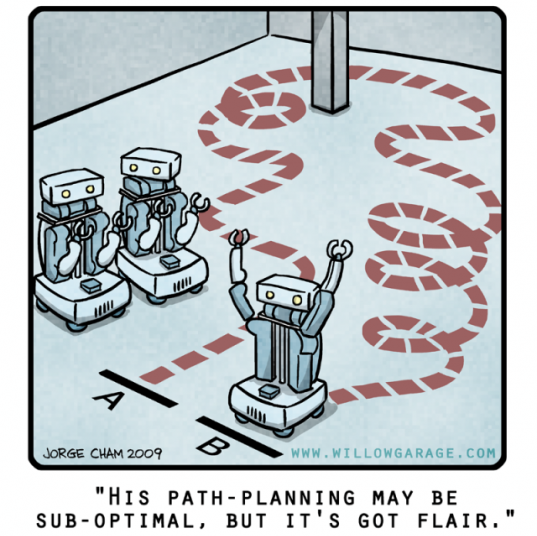
\includegraphics[width=\textwidth]{graphics/path-planning} \\
			\tiny\smallskip{Source: \url{http://www.willowgarage.com/blog/2009/09/04/robot-comics-path-planning}}
		\end{center}
	\end{column}
\end{columns}
\end{frame}

\subsection{Autonomous robotic vehicles and applications}
\begin{frame}
\frametitle{Introduction}
\begin{columns}
	\begin{column}{0.55\textwidth}
		\hspace{0.5cm} Guide a robot through the environment. \\[0.1cm]
		\hspace{1.2cm} \textbf{Mapping}. \\
		\hspace{1.2cm} \textbf{Traversability.} \\
		\hspace{1.2cm} \phantom{Localization.} \\
		\hspace{1.2cm} \phantom{Localization.} \\
	\end{column}
	\begin{column}{0.5\textwidth}
		\begin{center}
			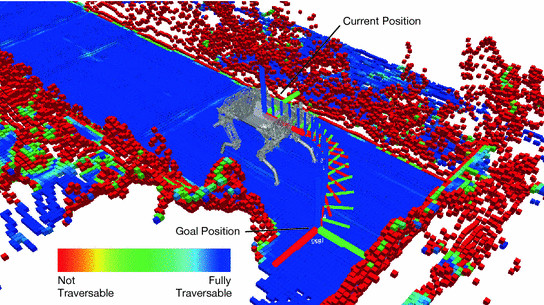
\includegraphics[width=\textwidth]{graphics/traversability.png} \\
			\tiny\smallskip{Source: Fankhauser and Hutter (2016)}
		\end{center}
	\end{column}
\end{columns}
\end{frame}

\subsection{Ground vs Aerial}
\begin{frame}
\frametitle{Introduction}
\begin{columns}
	\begin{column}{0.55\textwidth}
		\hspace{0.5cm} Guide a robot through the environment. \\[0.1cm]
		\hspace{1.2cm} \textbf{Mapping}. \\
		\hspace{1.2cm} \textbf{Traversability.} \\
		\hspace{1.2cm} \textbf{Aerial data.} \\
		\hspace{1.2cm} \phantom{Localization.} \\
	\end{column}
	\begin{column}{0.5\textwidth}
		\begin{center}
			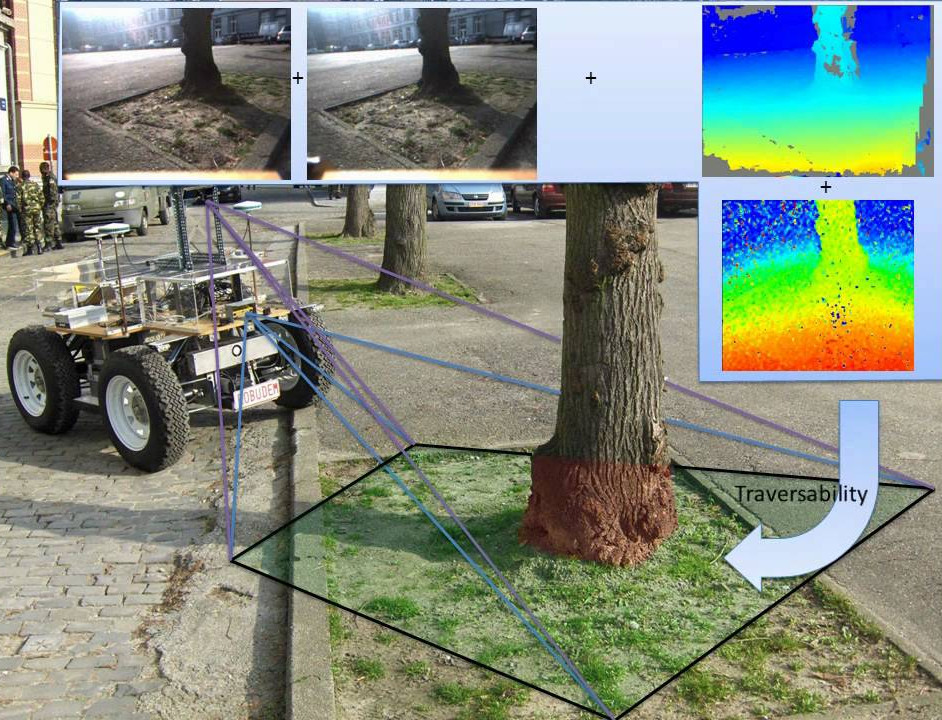
\includegraphics[width=0.75\textwidth]{graphics/trav-from-ground} \\
			\tiny\smallskip{Source: \url{https://www.youtube.com/watch?v=CNFc5qPvnB0}}
		\end{center}
		\begin{center}
			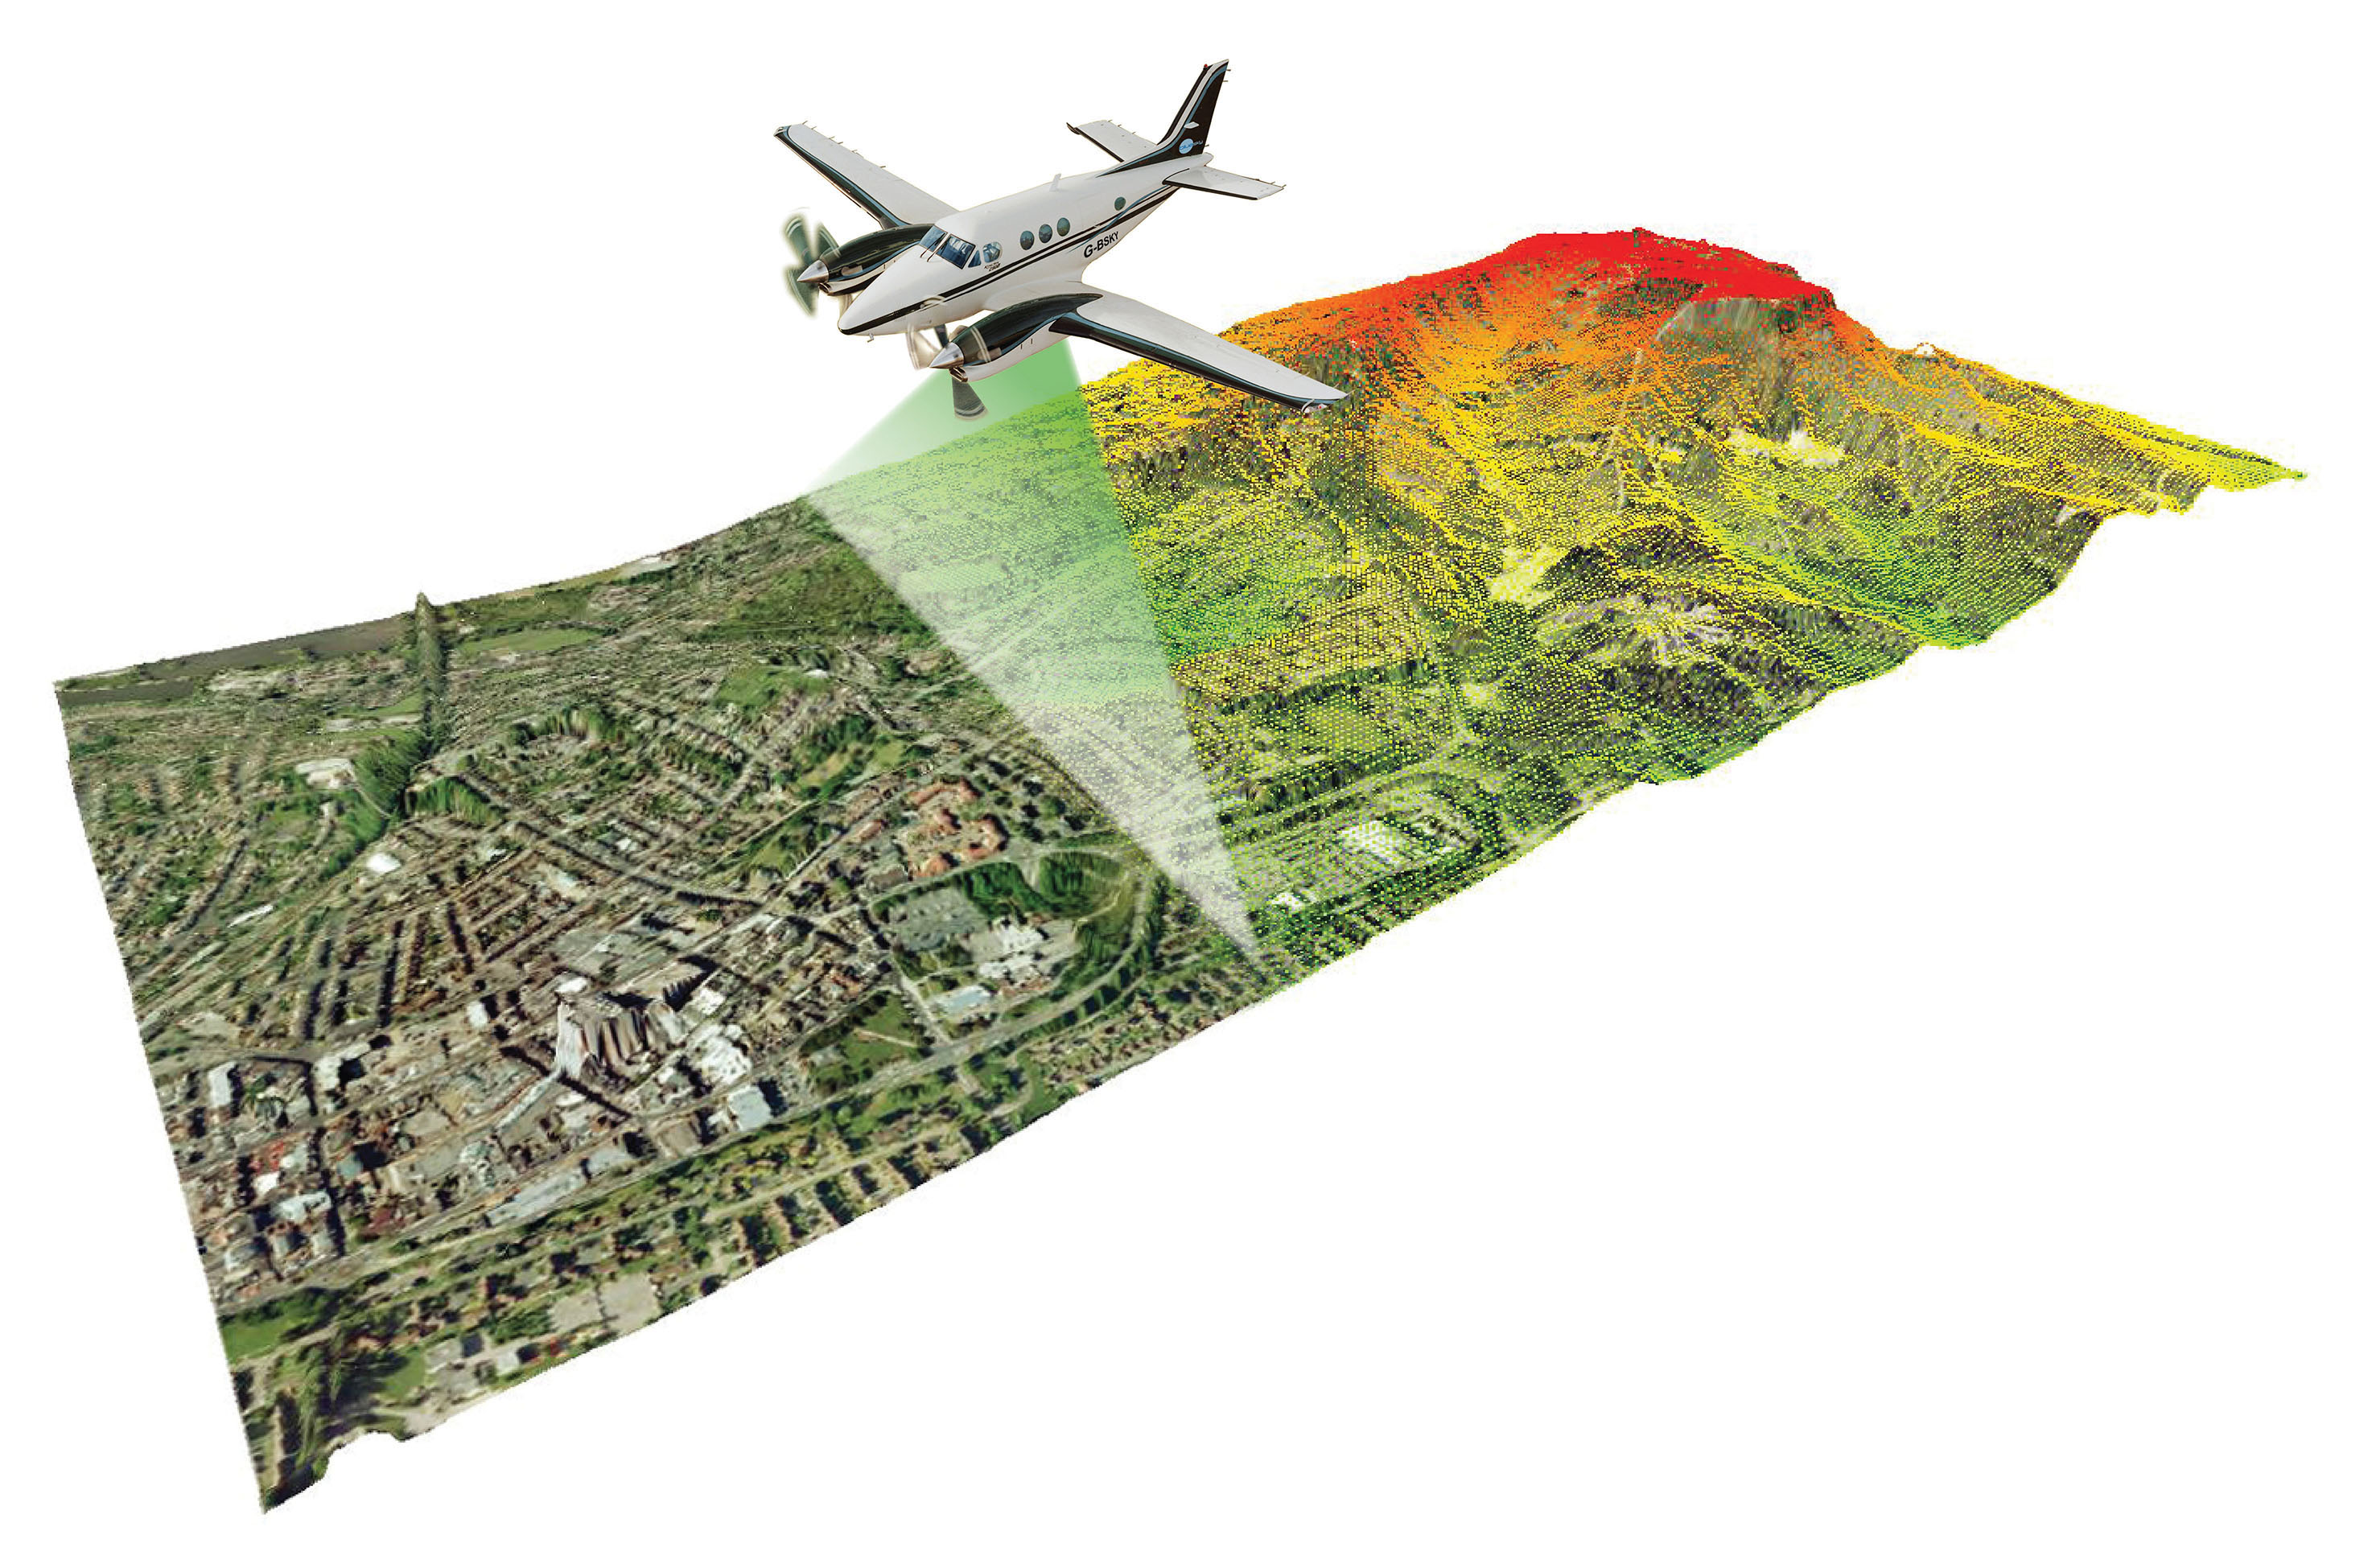
\includegraphics[width=0.8\textwidth]{graphics/lidar_data} \\
			\tiny\smallskip{Source: \url{https://www.directionsmag.com/pressrelease/6225}}
		\end{center}
	\end{column}
\end{columns}
\end{frame}

\begin{frame}
\frametitle{Goal}
\begin{exampleblock}{Main goal}
	Compute traversability maps from aerial data.
\end{exampleblock}
\begin{center}
	\begin{minipage}{0.45\textwidth}
		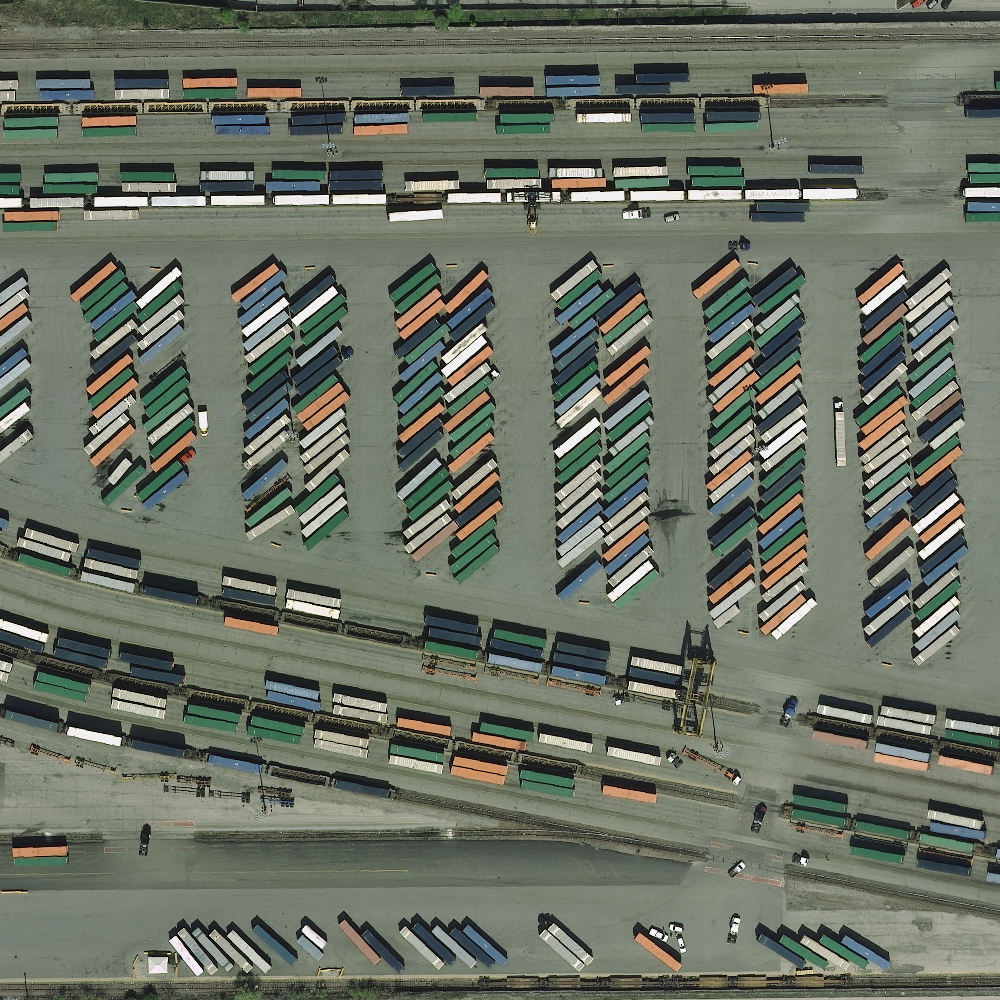
\includegraphics[width=\textwidth]{graphics/aerial04.jpg} \\
		\centering\tiny\smallskip{Source: Borges et al. (2019)}
	\end{minipage} \hspace{0.25cm}
	\begin{minipage}{0.45\textwidth}
		
\includegraphics[width=\textwidth]{graphics/aerial04-trav.jpg} \\
		\centering\tiny\smallskip{Source: Borges et al. (2019)}
	\end{minipage}
\end{center}
\end{frame}

\begin{frame}
\frametitle{Previous work}
\hspace{0.5cm}
\begin{minipage}[]{0.45\textwidth}
	\centering
	Image input \\
	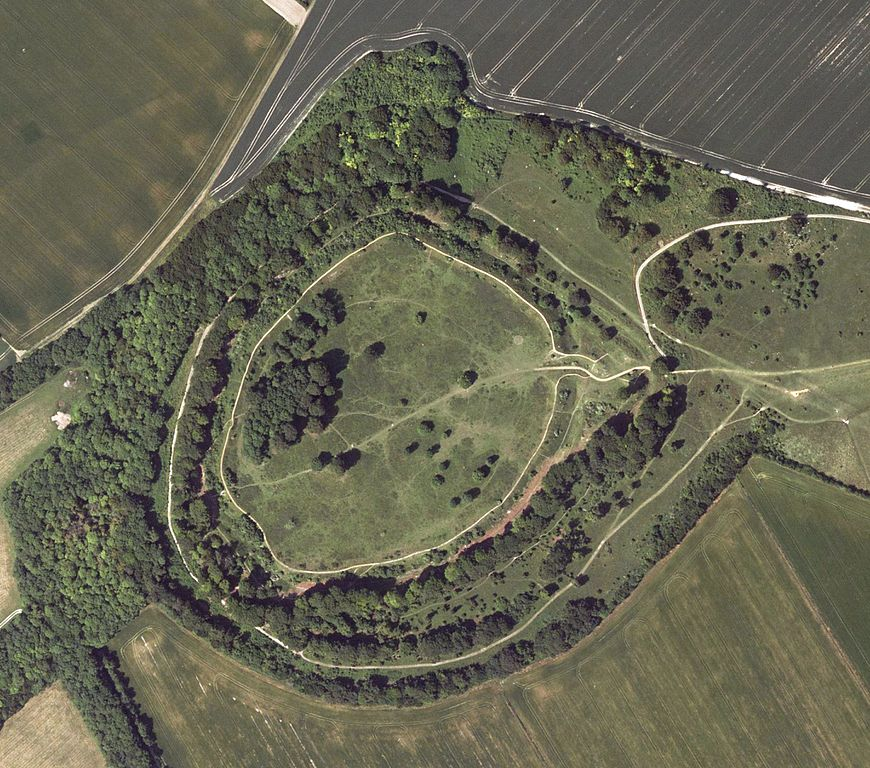
\includegraphics[width=0.6\textwidth]{graphics/aerial_image.jpg} \\
	\centering\tiny\smallskip{Source: \url{https://en.wikipedia.org/wiki/Hampshire}}
	\flushleft
	\scriptsize
	\hspace{0.75cm} Hudjakov and Tamre (2011) \\
	\hspace{0.75cm} Hudjakov and Tamre (2013) \\
	\hspace{0.75cm} Delmerico (2017) \\
	\hspace{0.75cm} Borges et al. (2019) \\
	\hspace{0.75cm} \phantom{Borges et al. (2019)} \\
\end{minipage}%
\begin{minipage}[]{0.45\textwidth}
	\centering
	Depth input \\
	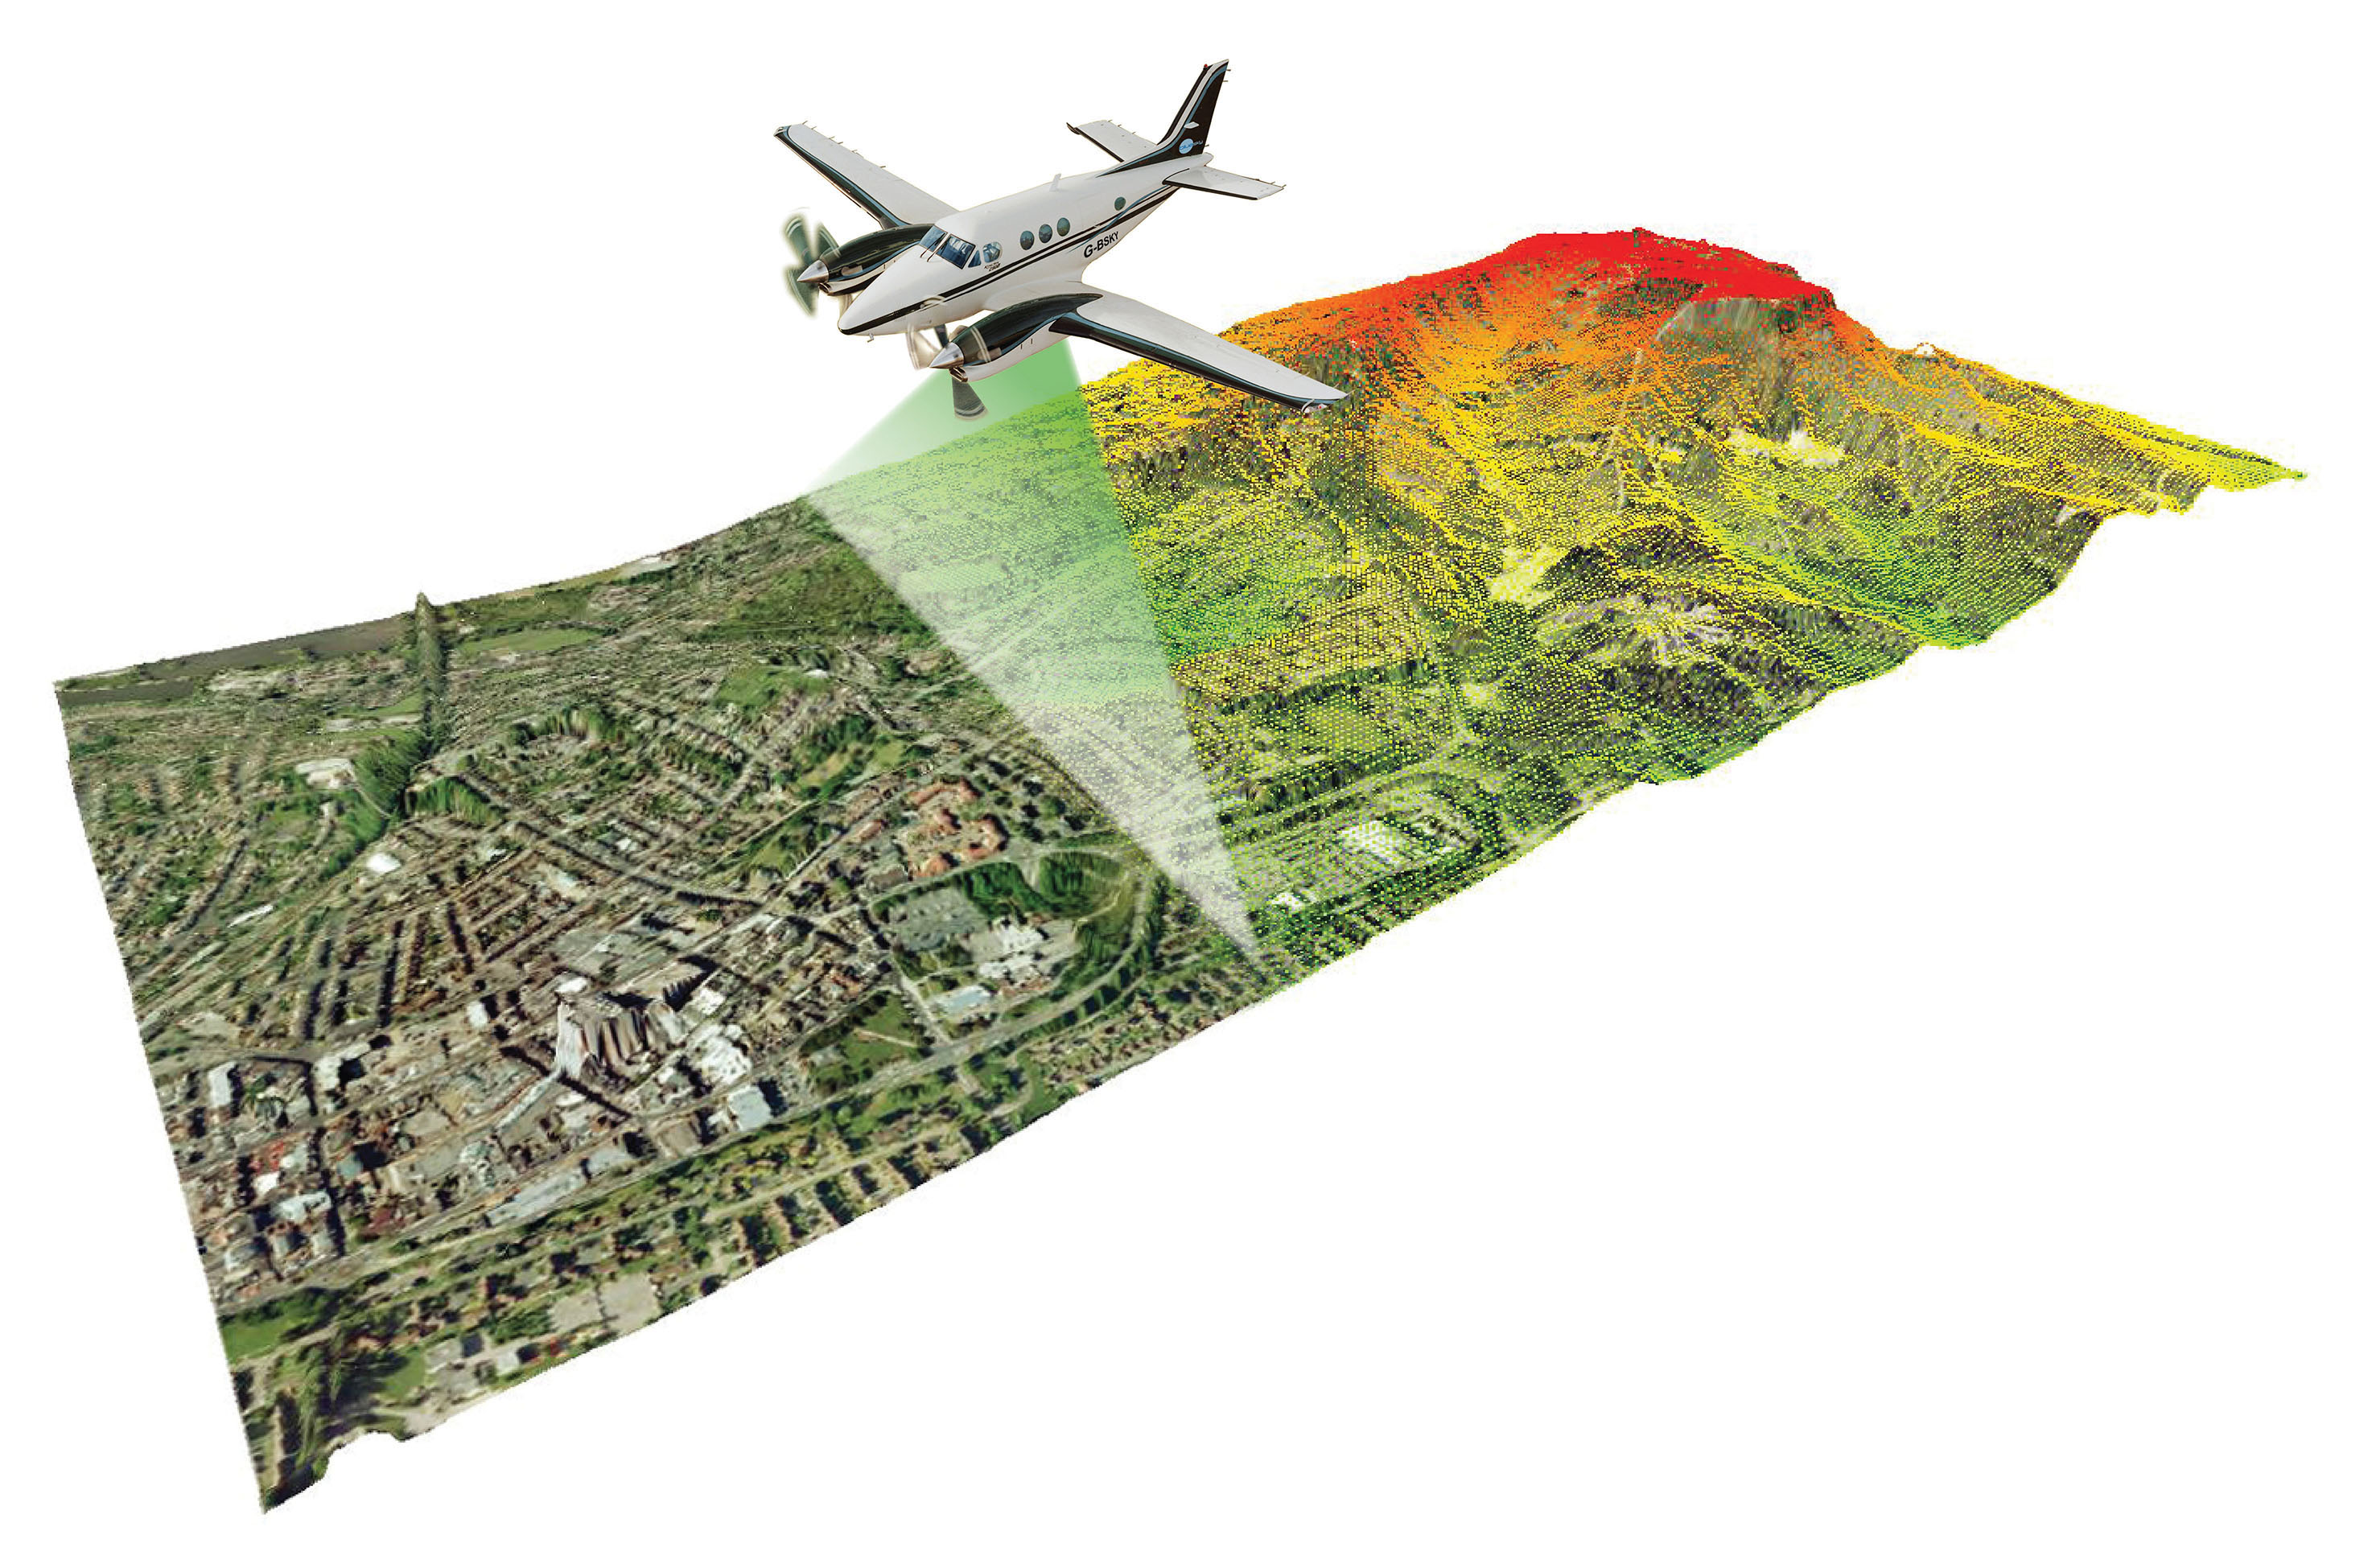
\includegraphics[width=0.79\textwidth]{graphics/lidar_data.jpg} \\
	\centering\tiny\smallskip{Source: \url{https://www.directionsmag.com/pressrelease/6225}}
	\flushleft
	\scriptsize
	\hspace{0.75cm} Vandapel et al. (2006) \\
	\hspace{0.75cm} Silver et al. (2006) \\
	\hspace{0.75cm} Sofman et al. (2006) \\
	\hspace{0.75cm} Shneier et al. (2008) \\
	\hspace{0.75cm} Chavez-Garcia et al. (2018) \\
\end{minipage}
\end{frame}

\begin{frame}
\frametitle{Previous work}
\centering
Traversability maps from image classification \\[0.5cm]
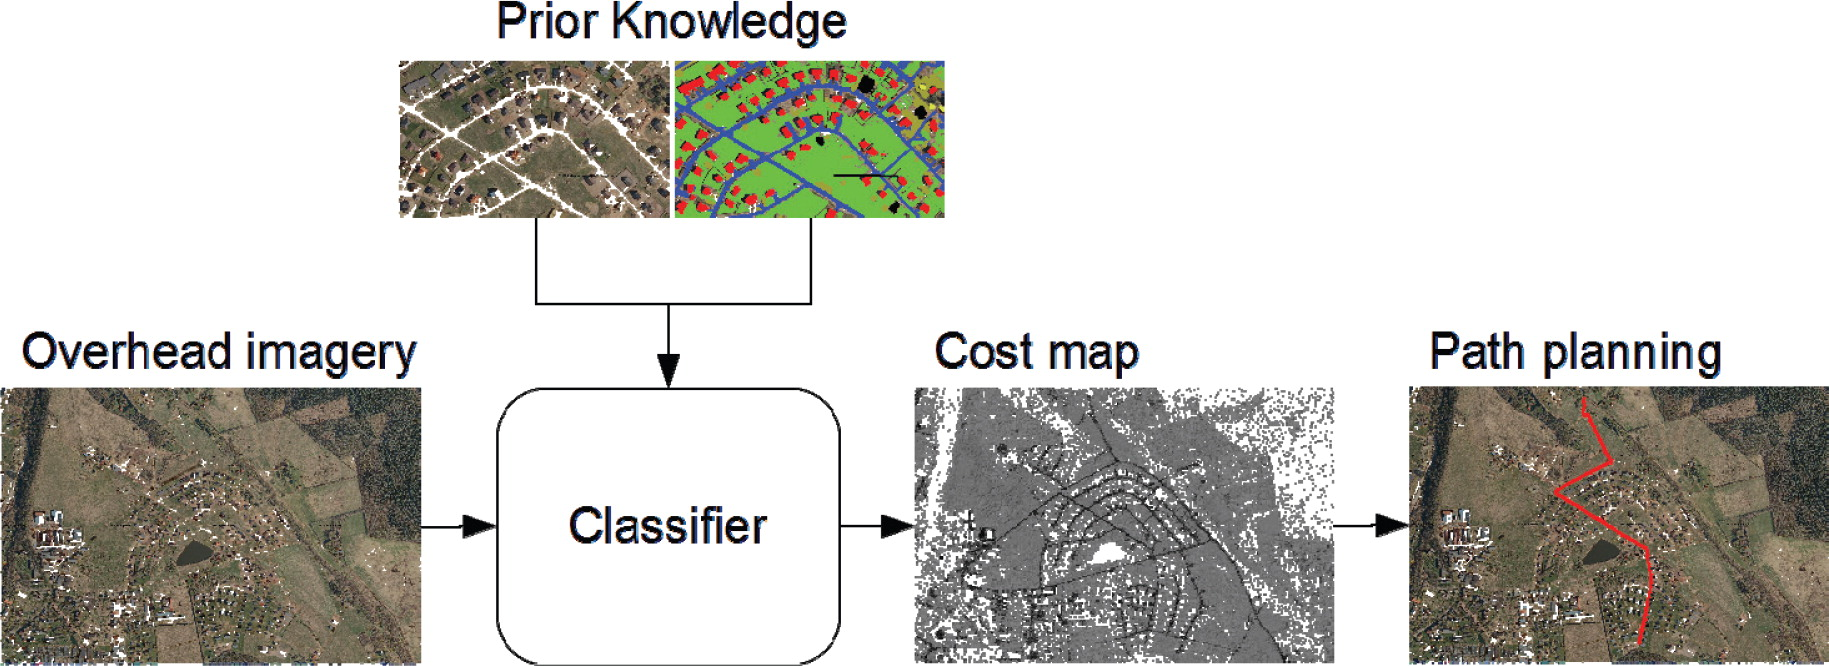
\includegraphics[width=\textwidth]{graphics/ht.jpg} \\
\centering\tiny\smallskip{Source: Hudjakov and Tamre (2013)}
\end{frame}

\begin{frame}
\frametitle{Previous work}
\centering
Traversability maps from heuristics \\[0.5cm]
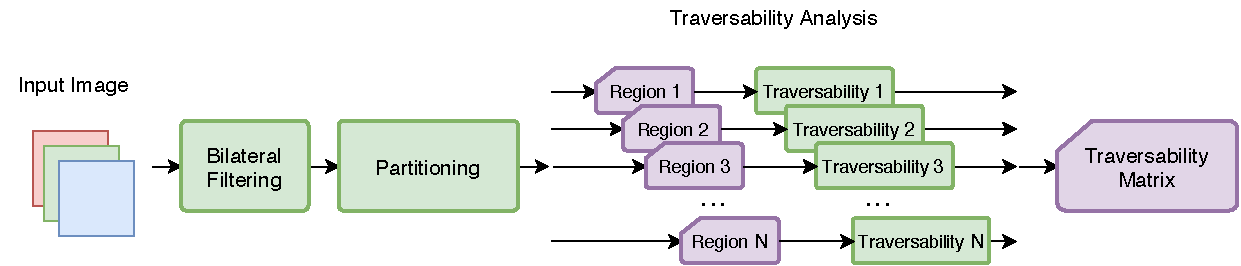
\includegraphics[width=\textwidth]{graphics/eswa-proposal-flowchart.pdf} \\
\centering\tiny\smallskip{Source: Borges et al. (2019)}
\end{frame}

\begin{frame}
\frametitle{Proposal}
\centering
Traversability maps from fully convolutional neural networks \\[0.5cm]
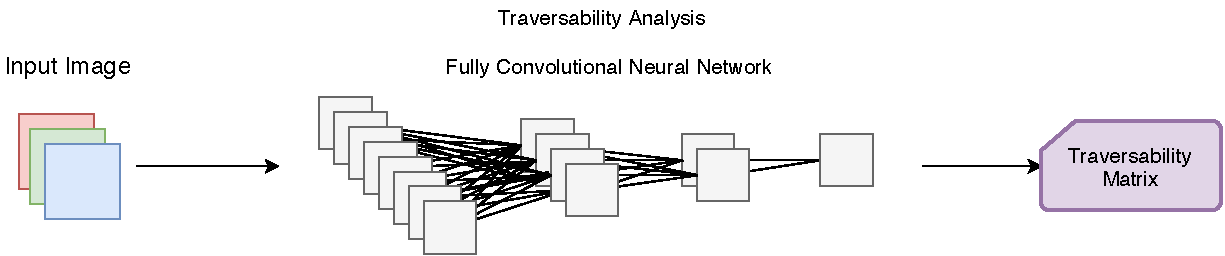
\includegraphics[width=\textwidth]{graphics/proposal-flowchart.pdf}
\end{frame}

\begin{frame}
\frametitle{TFCN architecture}
\hspace{0.5cm}
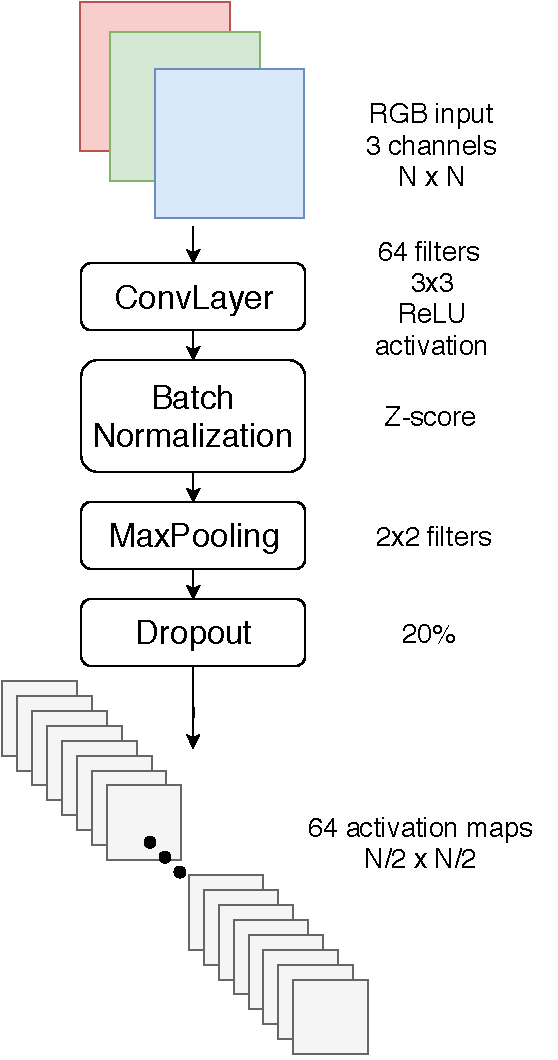
\includegraphics[width=0.3\textwidth]{graphics/TFCN1.pdf}
\hspace{0.12cm}
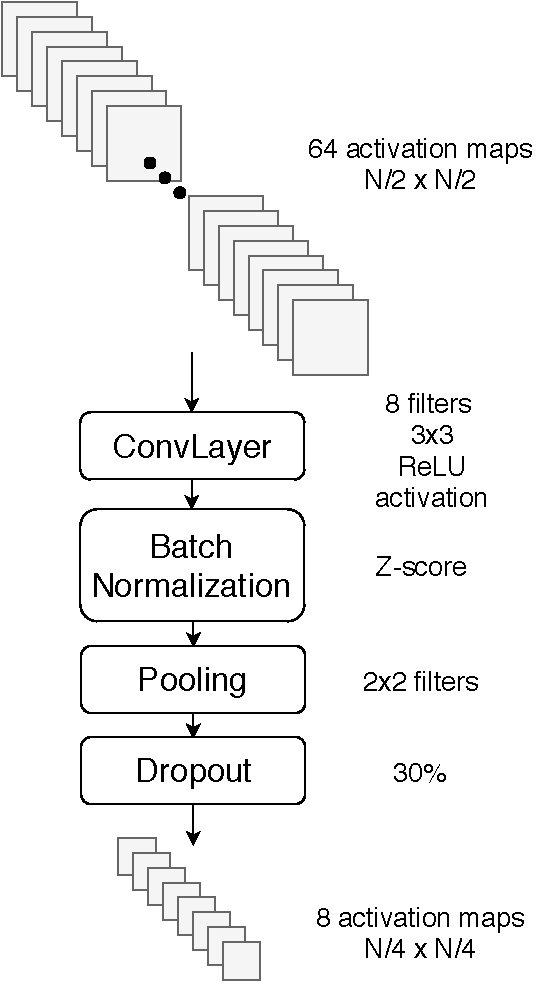
\includegraphics[width=0.3\textwidth]{graphics/TFCN2.pdf}
\hspace{0.12cm}
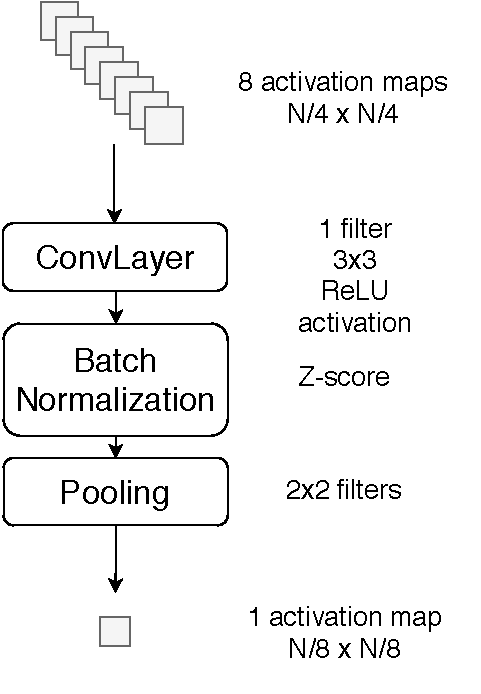
\includegraphics[width=0.3\textwidth]{graphics/TFCN3.pdf}
\end{frame}

\begin{frame}
\frametitle{Dataset}
\begin{description}
	\item[ATPD] Aerial Traversability and Planning Dataset.
	\item[Data] 8 aerial images and their traversability labels.
	\item[Image size] $1000 \times 1000$ pixels.
	\item[Resolution] $0.3\ m \times 0.3 \ m/p$.
\end{description}
\centering

\includegraphics[width=0.11\textwidth]{graphics/aerial01.jpg}

\includegraphics[width=0.11\textwidth]{graphics/aerial02.jpg}

\includegraphics[width=0.11\textwidth]{graphics/aerial03.jpg}
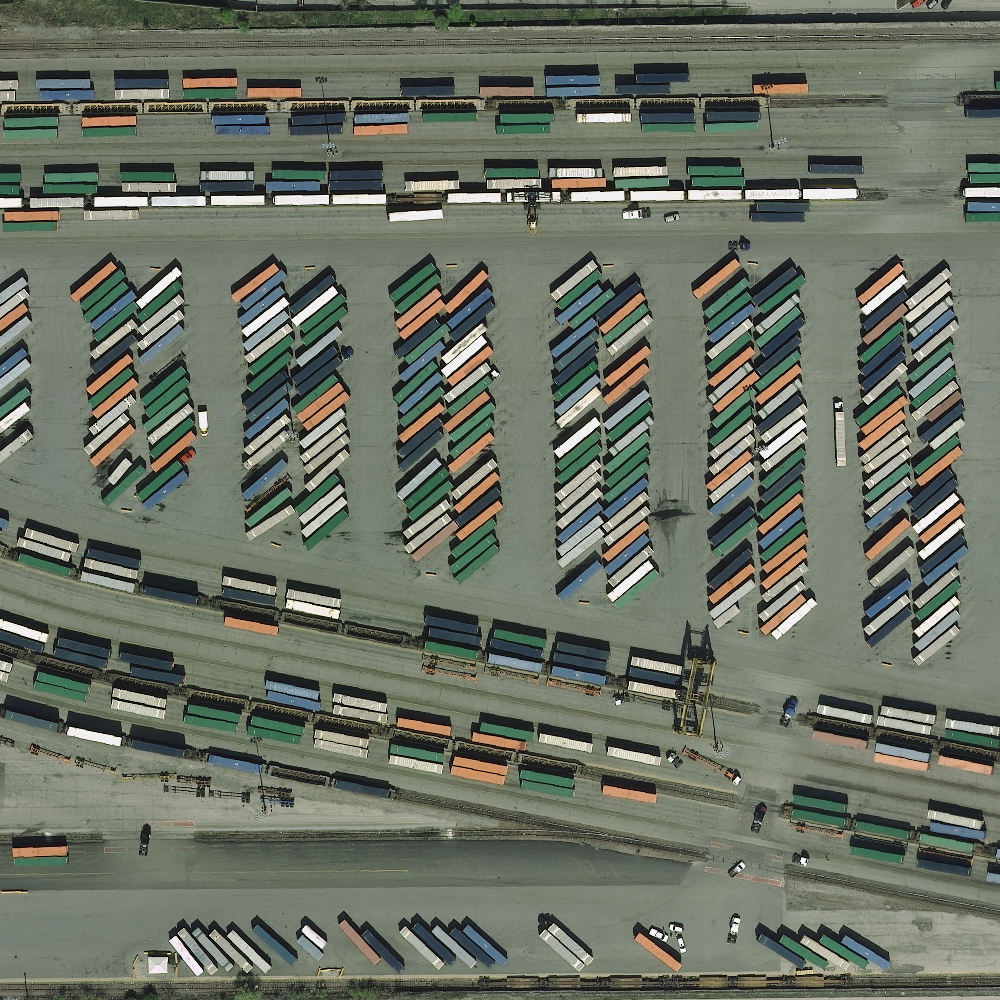
\includegraphics[width=0.11\textwidth]{graphics/aerial04.jpg}

\includegraphics[width=0.11\textwidth]{graphics/aerial05.jpg}
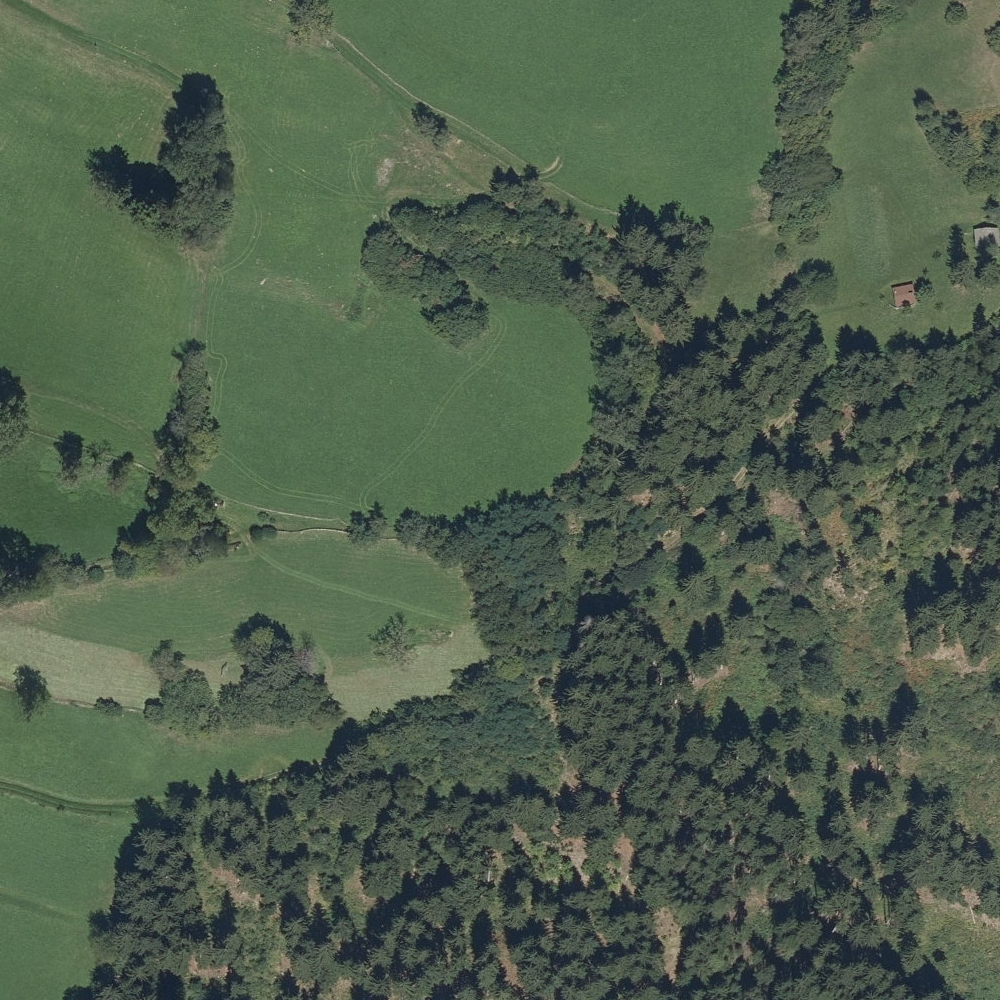
\includegraphics[width=0.11\textwidth]{graphics/aerial06.jpg}

\includegraphics[width=0.11\textwidth]{graphics/aerial07.jpg}

\includegraphics[width=0.11\textwidth]{graphics/aerial08.jpg}

\vspace{0.25cm}


\includegraphics[width=0.11\textwidth]{graphics/aerial01-trav.jpg}

\includegraphics[width=0.11\textwidth]{graphics/aerial02-trav.jpg}

\includegraphics[width=0.11\textwidth]{graphics/aerial03-trav.jpg}

\includegraphics[width=0.11\textwidth]{graphics/aerial04-trav.jpg}

\includegraphics[width=0.11\textwidth]{graphics/aerial05-trav.jpg}
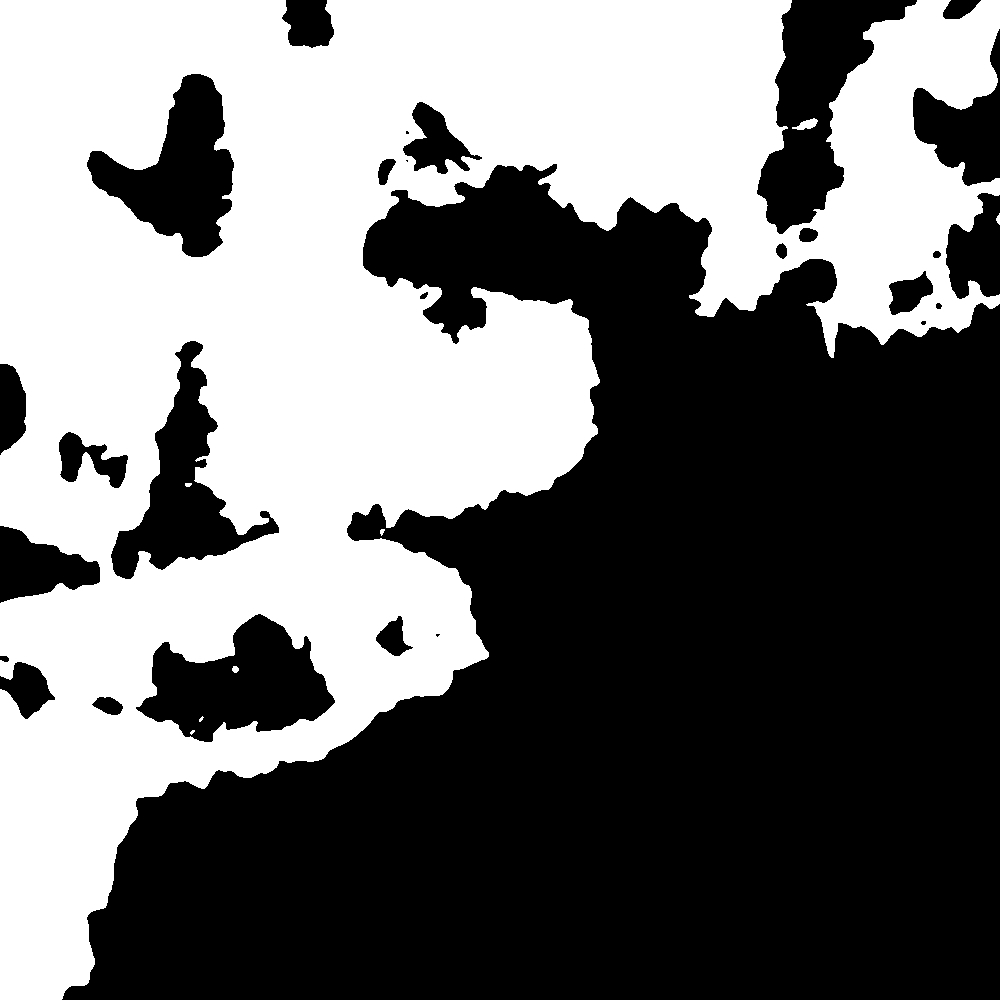
\includegraphics[width=0.11\textwidth]{graphics/aerial06-trav.jpg}
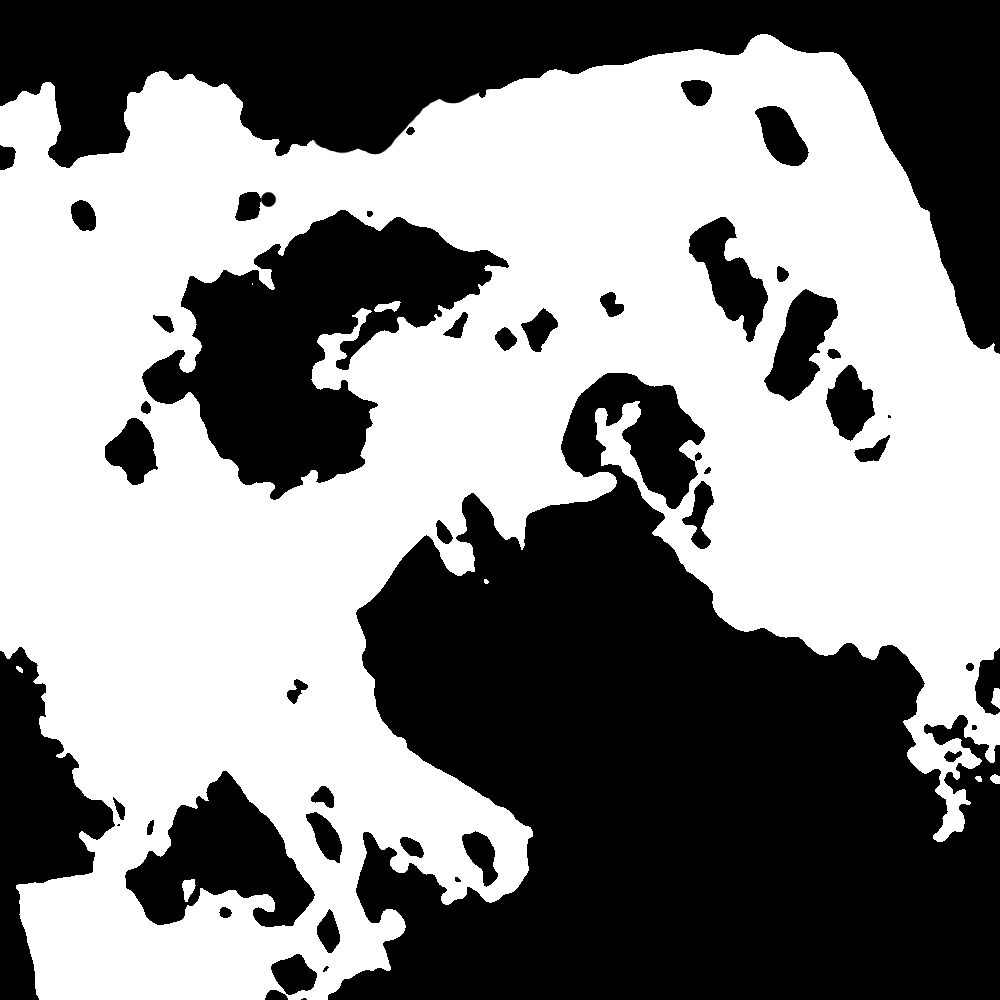
\includegraphics[width=0.11\textwidth]{graphics/aerial07-trav.jpg}

\includegraphics[width=0.11\textwidth]{graphics/aerial08-trav.jpg}

\centering\tiny\smallskip{Source: Borges et al. (2019)}
\end{frame}

\begin{frame}
\frametitle{Data augmentation}
\begin{description}
	\item[Rotations] Random angles from 0º to 360º.
	\item[Shifts] Max 30\% vertical and horizontal.
	\item[Flips] Vertical and horizontal.
	\item[Shear] Max 30º distortion.
	\item[Zoom] Max 20\% amplification.
\end{description}
\end{frame}

\begin{frame}
\frametitle{Training}
\begin{description}
	\item[Optmizer] Adam.
	\item[Loss function] Mean Squared Error.
	\item[Max epochs] 100.
	\item[Early stopping] if validation loss does not improve after 20 epochs.
\end{description}
\end{frame}

\begin{frame}
\frametitle{Cross-validation}

\newcommand{\test}{Red}
\newcommand{\train}{JungleGreen}
\newcommand{\val}{NavyBlue}
\fboxsep=0.6mm

\begin{minipage}[]{0.25\textwidth}
	\textbf{Leave-one-out} \\
	\textcolor{\test}{$\blacksquare$} 1 test image \\
	\textcolor{\val}{$\blacksquare$} 1 validation image \\
	\textcolor{\train}{$\blacksquare$} 6 training images
\end{minipage}%
\begin{minipage}[]{0.9\textwidth}
\centering
\fcolorbox{white}{\test}{
\includegraphics[width=0.06\textwidth]{graphics/aerial01.jpg}}
\fcolorbox{white}{\val}{
\includegraphics[width=0.06\textwidth]{graphics/aerial02.jpg}}
\fcolorbox{white}{\train}{
\includegraphics[width=0.06\textwidth]{graphics/aerial03.jpg}}
\fcolorbox{white}{\train}{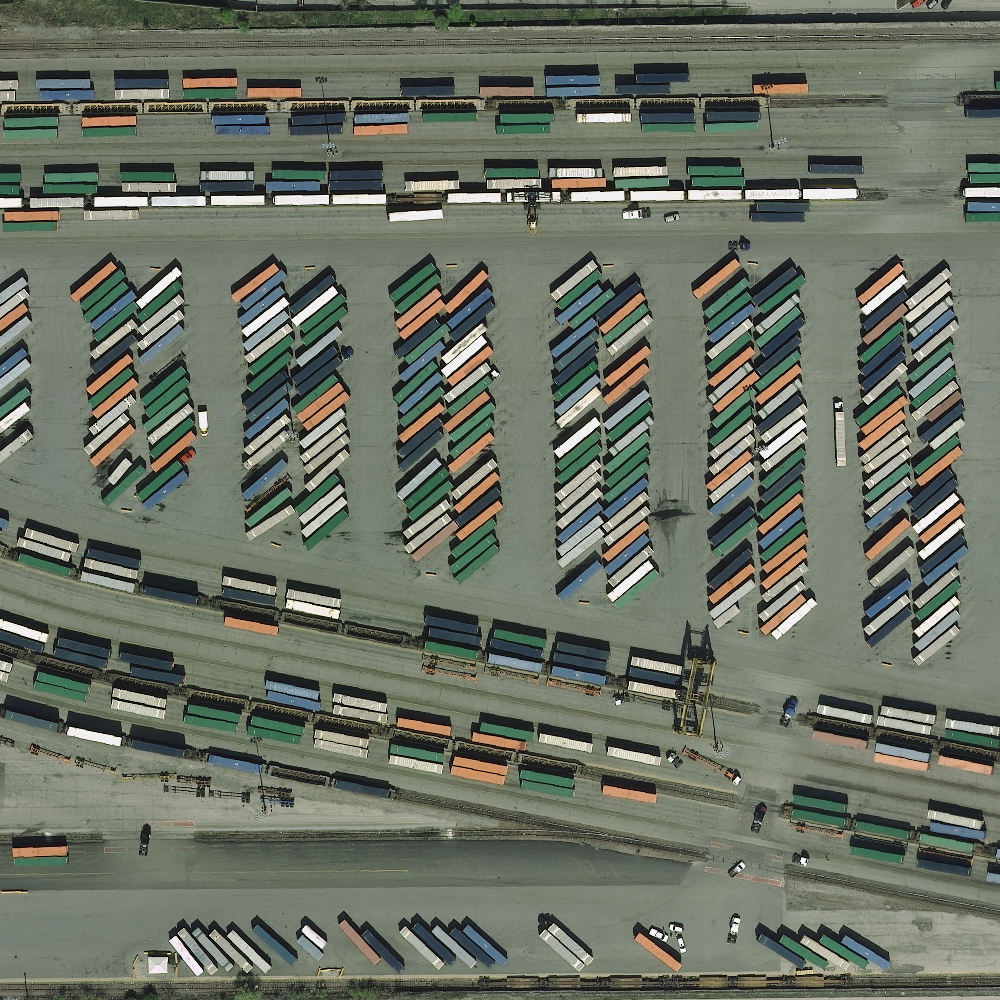
\includegraphics[width=0.06\textwidth]{graphics/aerial04.jpg}}
\fcolorbox{white}{\train}{
\includegraphics[width=0.06\textwidth]{graphics/aerial05.jpg}}
\fcolorbox{white}{\train}{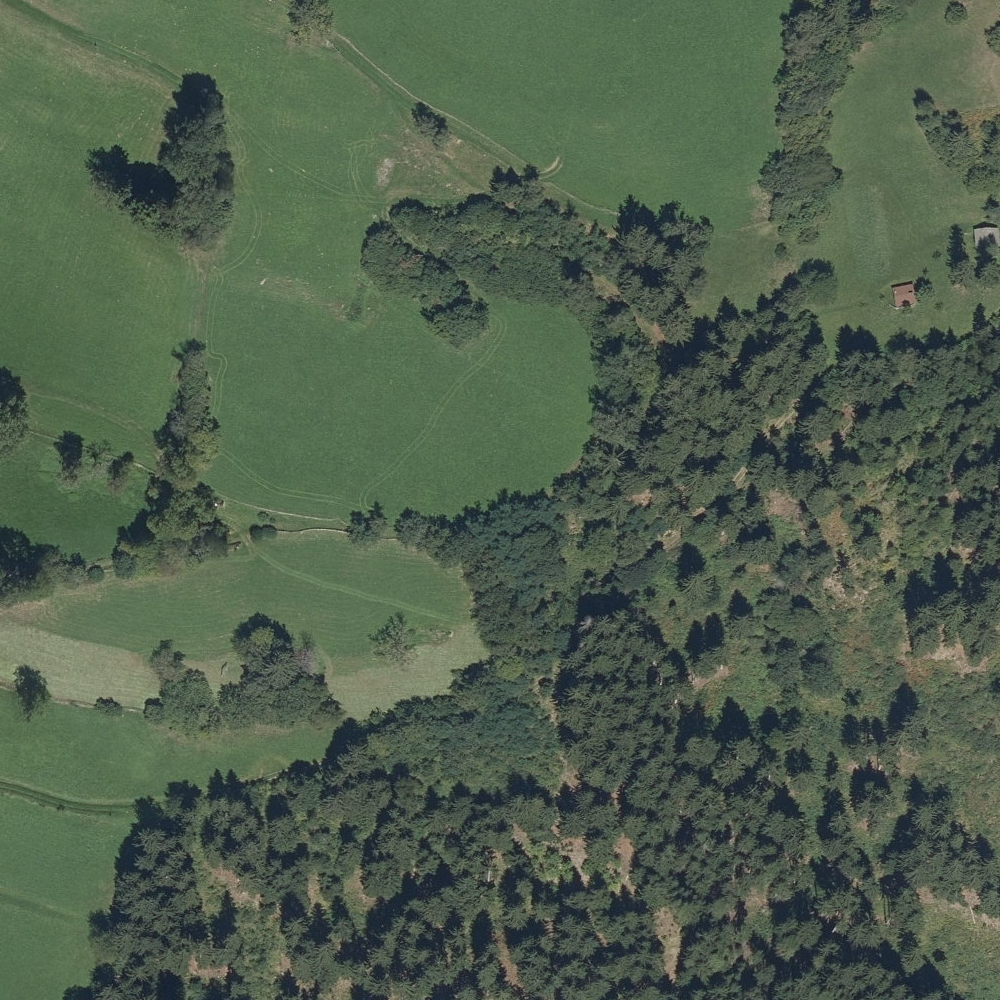
\includegraphics[width=0.06\textwidth]{graphics/aerial06.jpg}}
\fcolorbox{white}{\train}{
\includegraphics[width=0.06\textwidth]{graphics/aerial07.jpg}}
\fcolorbox{white}{\train}{
\includegraphics[width=0.06\textwidth]{graphics/aerial08.jpg}}

\fcolorbox{white}{\train}{
\includegraphics[width=0.06\textwidth]{graphics/aerial01.jpg}}
\fcolorbox{white}{\test}{
\includegraphics[width=0.06\textwidth]{graphics/aerial02.jpg}}
\fcolorbox{white}{\val}{
\includegraphics[width=0.06\textwidth]{graphics/aerial03.jpg}}
\fcolorbox{white}{\train}{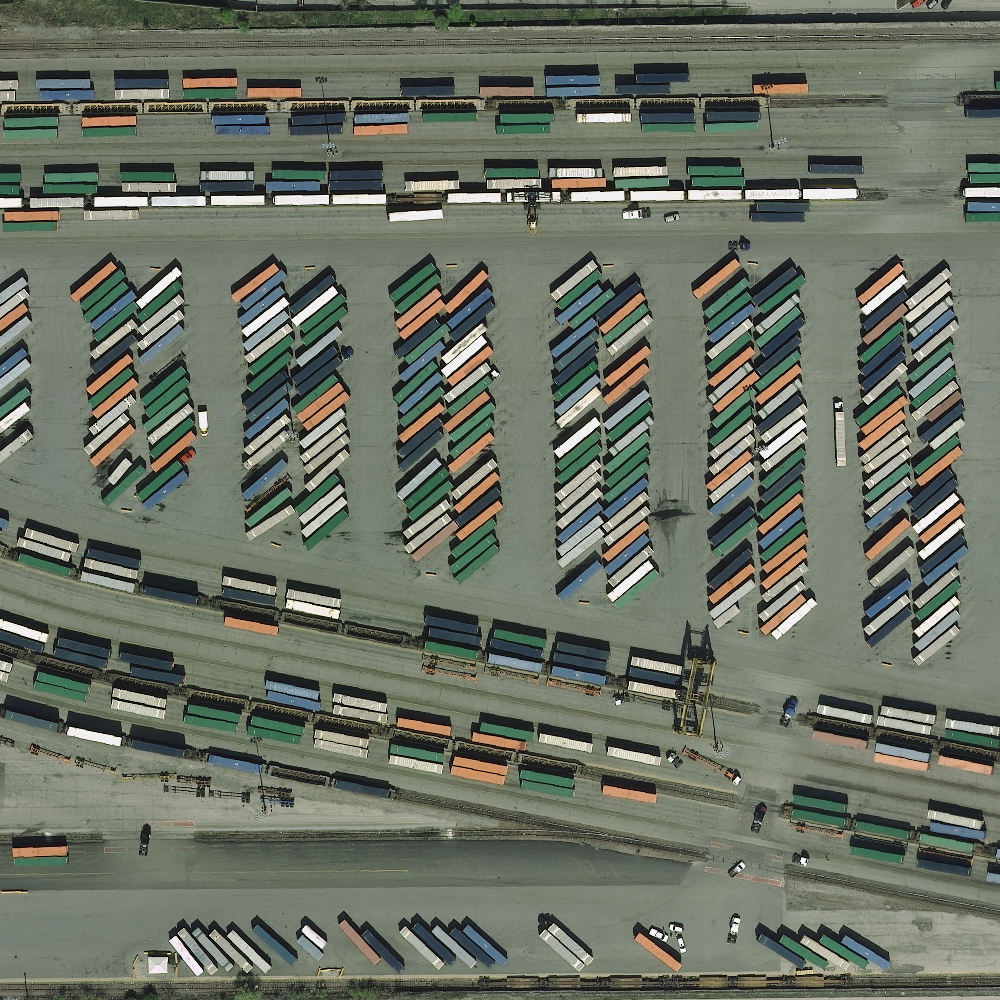
\includegraphics[width=0.06\textwidth]{graphics/aerial04.jpg}}
\fcolorbox{white}{\train}{
\includegraphics[width=0.06\textwidth]{graphics/aerial05.jpg}}
\fcolorbox{white}{\train}{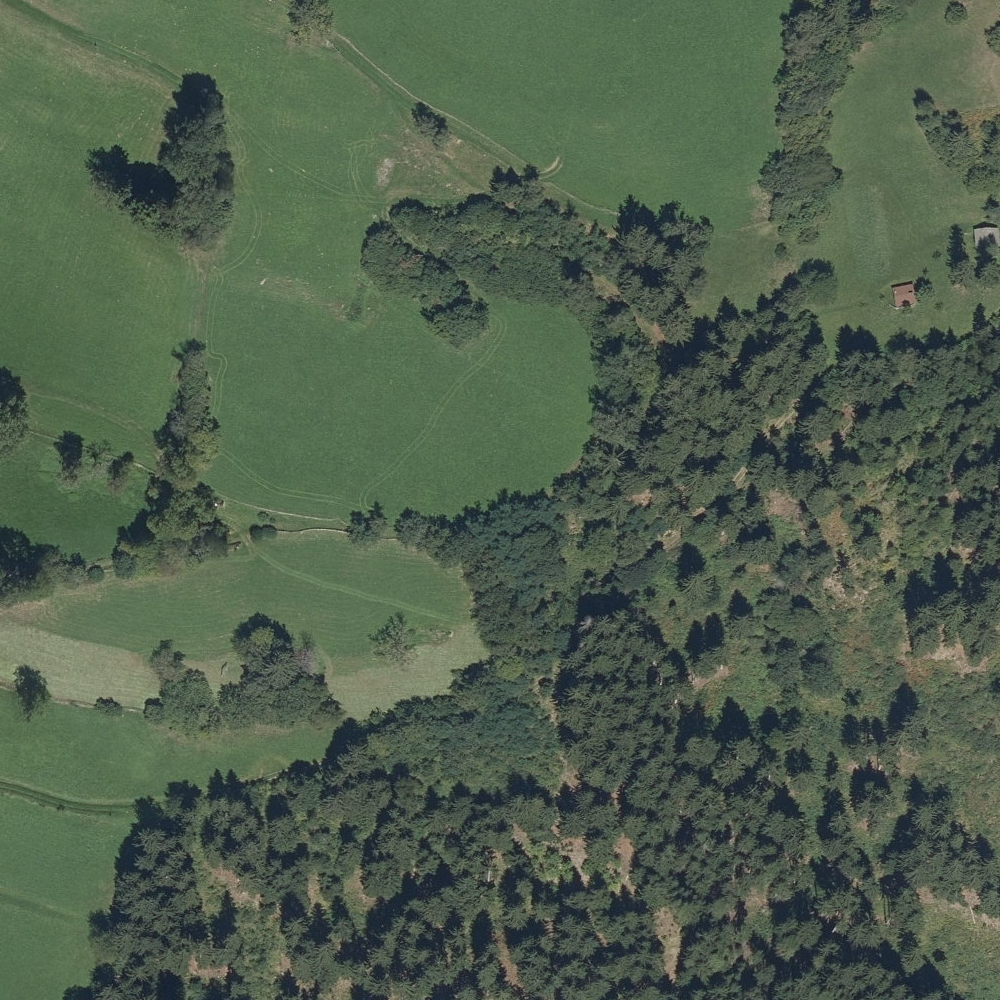
\includegraphics[width=0.06\textwidth]{graphics/aerial06.jpg}}
\fcolorbox{white}{\train}{
\includegraphics[width=0.06\textwidth]{graphics/aerial07.jpg}}
\fcolorbox{white}{\train}{
\includegraphics[width=0.06\textwidth]{graphics/aerial08.jpg}}

\fcolorbox{white}{\train}{
\includegraphics[width=0.06\textwidth]{graphics/aerial01.jpg}}
\fcolorbox{white}{\train}{
\includegraphics[width=0.06\textwidth]{graphics/aerial02.jpg}}
\fcolorbox{white}{\test}{
\includegraphics[width=0.06\textwidth]{graphics/aerial03.jpg}}
\fcolorbox{white}{\val}{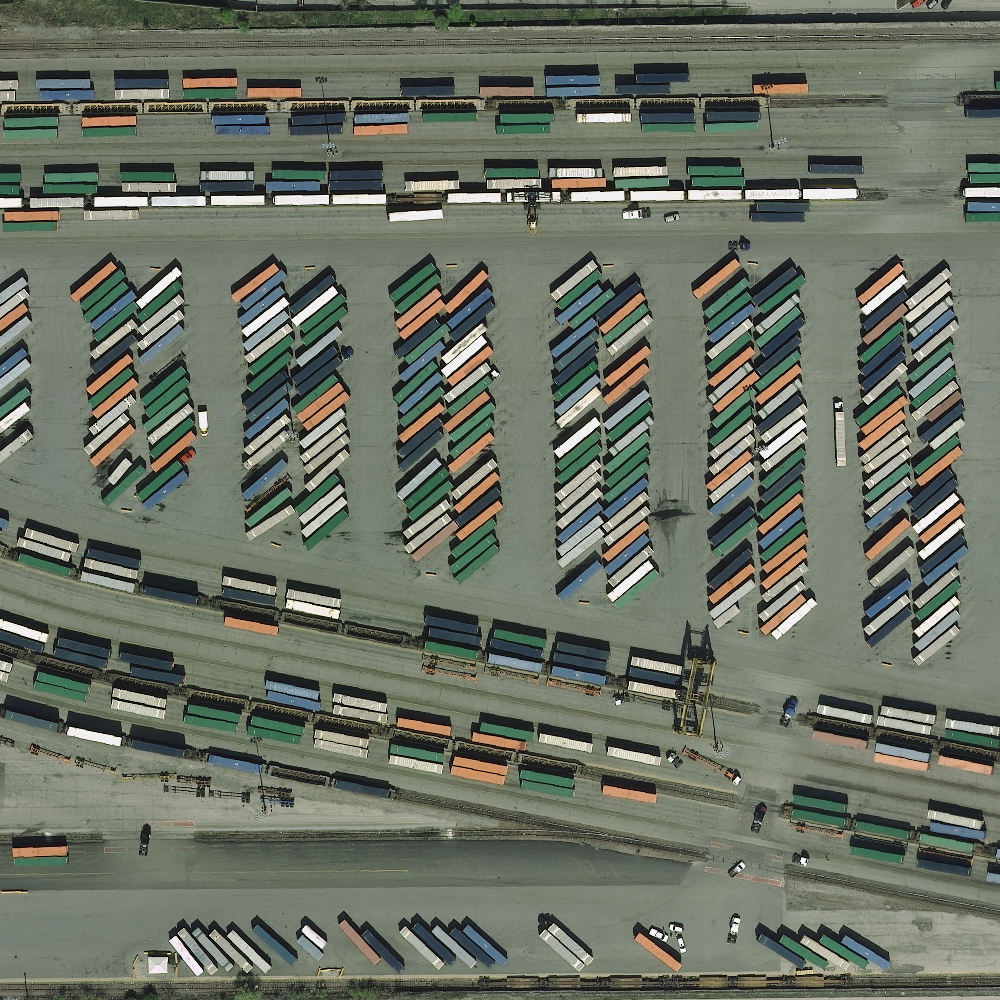
\includegraphics[width=0.06\textwidth]{graphics/aerial04.jpg}}
\fcolorbox{white}{\train}{\includegraphics[width=0.06\textwidth]{graphics/aerial05.jpg}}
\fcolorbox{white}{\train}{\includegraphics[width=0.06\textwidth]{graphics/aerial06.jpg}}
\fcolorbox{white}{\train}{\includegraphics[width=0.06\textwidth]{graphics/aerial07.jpg}}
\fcolorbox{white}{\train}{\includegraphics[width=0.06\textwidth]{graphics/aerial08.jpg}}

\fcolorbox{white}{\train}{\includegraphics[width=0.06\textwidth]{graphics/aerial01.jpg}}
\fcolorbox{white}{\train}{\includegraphics[width=0.06\textwidth]{graphics/aerial02.jpg}}
\fcolorbox{white}{\train}{\includegraphics[width=0.06\textwidth]{graphics/aerial03.jpg}}
\fcolorbox{white}{\test}{\includegraphics[width=0.06\textwidth]{graphics/aerial04.jpg}}
\fcolorbox{white}{\val}{\includegraphics[width=0.06\textwidth]{graphics/aerial05.jpg}}
\fcolorbox{white}{\train}{\includegraphics[width=0.06\textwidth]{graphics/aerial06.jpg}}
\fcolorbox{white}{\train}{\includegraphics[width=0.06\textwidth]{graphics/aerial07.jpg}}
\fcolorbox{white}{\train}{\includegraphics[width=0.06\textwidth]{graphics/aerial08.jpg}}

\fcolorbox{white}{\train}{\includegraphics[width=0.06\textwidth]{graphics/aerial01.jpg}}
\fcolorbox{white}{\train}{\includegraphics[width=0.06\textwidth]{graphics/aerial02.jpg}}
\fcolorbox{white}{\train}{\includegraphics[width=0.06\textwidth]{graphics/aerial03.jpg}}
\fcolorbox{white}{\train}{\includegraphics[width=0.06\textwidth]{graphics/aerial04.jpg}}
\fcolorbox{white}{\test}{\includegraphics[width=0.06\textwidth]{graphics/aerial05.jpg}}
\fcolorbox{white}{\val}{\includegraphics[width=0.06\textwidth]{graphics/aerial06.jpg}}
\fcolorbox{white}{\train}{\includegraphics[width=0.06\textwidth]{graphics/aerial07.jpg}}
\fcolorbox{white}{\train}{\includegraphics[width=0.06\textwidth]{graphics/aerial08.jpg}}

\fcolorbox{white}{\train}{\includegraphics[width=0.06\textwidth]{graphics/aerial01.jpg}}
\fcolorbox{white}{\train}{\includegraphics[width=0.06\textwidth]{graphics/aerial02.jpg}}
\fcolorbox{white}{\train}{\includegraphics[width=0.06\textwidth]{graphics/aerial03.jpg}}
\fcolorbox{white}{\train}{\includegraphics[width=0.06\textwidth]{graphics/aerial04.jpg}}
\fcolorbox{white}{\train}{\includegraphics[width=0.06\textwidth]{graphics/aerial05.jpg}}
\fcolorbox{white}{\test}{\includegraphics[width=0.06\textwidth]{graphics/aerial06.jpg}}
\fcolorbox{white}{\val}{\includegraphics[width=0.06\textwidth]{graphics/aerial07.jpg}}
\fcolorbox{white}{\train}{\includegraphics[width=0.06\textwidth]{graphics/aerial08.jpg}}

\fcolorbox{white}{\train}{\includegraphics[width=0.06\textwidth]{graphics/aerial01.jpg}}
\fcolorbox{white}{\train}{\includegraphics[width=0.06\textwidth]{graphics/aerial02.jpg}}
\fcolorbox{white}{\train}{\includegraphics[width=0.06\textwidth]{graphics/aerial03.jpg}}
\fcolorbox{white}{\train}{\includegraphics[width=0.06\textwidth]{graphics/aerial04.jpg}}
\fcolorbox{white}{\train}{\includegraphics[width=0.06\textwidth]{graphics/aerial05.jpg}}
\fcolorbox{white}{\train}{\includegraphics[width=0.06\textwidth]{graphics/aerial06.jpg}}
\fcolorbox{white}{\test}{\includegraphics[width=0.06\textwidth]{graphics/aerial07.jpg}}
\fcolorbox{white}{\val}{\includegraphics[width=0.06\textwidth]{graphics/aerial08.jpg}}

\fcolorbox{white}{\val}{\includegraphics[width=0.06\textwidth]{graphics/aerial01.jpg}}
\fcolorbox{white}{\train}{\includegraphics[width=0.06\textwidth]{graphics/aerial02.jpg}}
\fcolorbox{white}{\train}{\includegraphics[width=0.06\textwidth]{graphics/aerial03.jpg}}
\fcolorbox{white}{\train}{\includegraphics[width=0.06\textwidth]{graphics/aerial04.jpg}}
\fcolorbox{white}{\train}{\includegraphics[width=0.06\textwidth]{graphics/aerial05.jpg}}
\fcolorbox{white}{\train}{\includegraphics[width=0.06\textwidth]{graphics/aerial06.jpg}}
\fcolorbox{white}{\train}{\includegraphics[width=0.06\textwidth]{graphics/aerial07.jpg}}
\fcolorbox{white}{\test}{\includegraphics[width=0.06\textwidth]{graphics/aerial08.jpg}}
\end{minipage}

\end{frame}

\begin{frame}
\frametitle{Results}
\begin{minipage}[]{0.3\textwidth}
\centering
Loss
\includegraphics[width=\textwidth]{graphics/loss01.pdf}
\end{minipage}
\hspace{0.25cm}
\begin{minipage}[]{0.3\textwidth}
\centering
Input
\includegraphics[width=\textwidth]{graphics/aerial01.jpg}
\end{minipage}
\hspace{0.25cm}
\begin{minipage}[]{0.3\textwidth}
\centering
Traversability Label
\includegraphics[width=\textwidth]{graphics/aerial01-trav.jpg}
\end{minipage} \\
\vspace{0.25cm}
\begin{minipage}[]{0.666\textwidth}
\includegraphics[width=\textwidth]{graphics/tfcn2.pdf}
\end{minipage}
\begin{minipage}[]{0.3\textwidth}
\centering
TFCN Output
\includegraphics[width=\textwidth]{graphics/tfcn-output-01.jpg}
\end{minipage}
\end{frame}

\begin{frame}
\frametitle{Results}
\begin{minipage}[]{0.3\textwidth}
\centering
Loss
\includegraphics[width=\textwidth]{graphics/loss02.pdf}
\end{minipage}
\hspace{0.25cm}
\begin{minipage}[]{0.3\textwidth}
\centering
Input
\includegraphics[width=\textwidth]{graphics/aerial02.jpg}
\end{minipage}
\hspace{0.25cm}
\begin{minipage}[]{0.3\textwidth}
\centering
Traversability Label
\includegraphics[width=\textwidth]{graphics/aerial02-trav.jpg}
\end{minipage} \\
\vspace{0.25cm}
\begin{minipage}[]{0.666\textwidth}
\includegraphics[width=\textwidth]{graphics/tfcn2.pdf}
\end{minipage}
\begin{minipage}[]{0.3\textwidth}
\centering
TFCN Output
\includegraphics[width=\textwidth]{graphics/tfcn-output-02.jpg}
\end{minipage}
\end{frame}

\begin{frame}
\frametitle{Results}
\begin{minipage}[]{0.3\textwidth}
	\centering
	Loss
	\includegraphics[width=\textwidth]{graphics/loss03.pdf}
\end{minipage}
\hspace{0.25cm}
\begin{minipage}[]{0.3\textwidth}
	\centering
	Input
	\includegraphics[width=\textwidth]{graphics/aerial03.jpg}
\end{minipage}
\hspace{0.25cm}
\begin{minipage}[]{0.3\textwidth}
	\centering
	Traversability Label
	\includegraphics[width=\textwidth]{graphics/aerial03-trav.jpg}
\end{minipage} \\
\vspace{0.25cm}
\begin{minipage}[]{0.666\textwidth}
	\includegraphics[width=\textwidth]{graphics/tfcn2.pdf}
\end{minipage}
\begin{minipage}[]{0.3\textwidth}
	\centering
	TFCN Output
	\includegraphics[width=\textwidth]{graphics/tfcn-output-03.jpg}
\end{minipage}
\end{frame}

\begin{frame}
\frametitle{Results}
\begin{minipage}[]{0.3\textwidth}
	\centering
	Loss
	\includegraphics[width=\textwidth]{graphics/loss04.pdf}
\end{minipage}
\hspace{0.25cm}
\begin{minipage}[]{0.3\textwidth}
	\centering
	Input
	\includegraphics[width=\textwidth]{graphics/aerial04.jpg}
\end{minipage}
\hspace{0.25cm}
\begin{minipage}[]{0.3\textwidth}
	\centering
	Traversability Label
	\includegraphics[width=\textwidth]{graphics/aerial04-trav.jpg}
\end{minipage} \\
\vspace{0.25cm}
\begin{minipage}[]{0.666\textwidth}
	\includegraphics[width=\textwidth]{graphics/tfcn2.pdf}
\end{minipage}
\begin{minipage}[]{0.3\textwidth}
	\centering
	TFCN Output
	\includegraphics[width=\textwidth]{graphics/tfcn-output-04.jpg}
\end{minipage}
\end{frame}

\begin{frame}
\frametitle{Results}
\begin{minipage}[]{0.3\textwidth}
	\centering
	Loss
	\includegraphics[width=\textwidth]{graphics/loss05.pdf}
\end{minipage}
\hspace{0.25cm}
\begin{minipage}[]{0.3\textwidth}
	\centering
	Input
	\includegraphics[width=\textwidth]{graphics/aerial05.jpg}
\end{minipage}
\hspace{0.25cm}
\begin{minipage}[]{0.3\textwidth}
	\centering
	Traversability Label
	\includegraphics[width=\textwidth]{graphics/aerial05-trav.jpg}
\end{minipage} \\
\vspace{0.25cm}
\begin{minipage}[]{0.666\textwidth}
	\includegraphics[width=\textwidth]{graphics/tfcn2.pdf}
\end{minipage}
\begin{minipage}[]{0.3\textwidth}
	\centering
	TFCN Output
	\includegraphics[width=\textwidth]{graphics/tfcn-output-05.jpg}
\end{minipage}
\end{frame}

\begin{frame}
\frametitle{Results}
\begin{minipage}[]{0.3\textwidth}
	\centering
	Loss
	\includegraphics[width=\textwidth]{graphics/loss06.pdf}
\end{minipage}
\hspace{0.25cm}
\begin{minipage}[]{0.3\textwidth}
	\centering
	Input
	\includegraphics[width=\textwidth]{graphics/aerial06.jpg}
\end{minipage}
\hspace{0.25cm}
\begin{minipage}[]{0.3\textwidth}
	\centering
	Traversability Label
	\includegraphics[width=\textwidth]{graphics/aerial06-trav.jpg}
\end{minipage} \\
\vspace{0.25cm}
\begin{minipage}[]{0.666\textwidth}
	\includegraphics[width=\textwidth]{graphics/tfcn2.pdf}
\end{minipage}
\begin{minipage}[]{0.3\textwidth}
	\centering
	TFCN Output
	\includegraphics[width=\textwidth]{graphics/tfcn-output-06.jpg}
\end{minipage}
\end{frame}

\begin{frame}
\frametitle{Results}
\begin{minipage}[]{0.3\textwidth}
	\centering
	Loss
	\includegraphics[width=\textwidth]{graphics/loss07.pdf}
\end{minipage}
\hspace{0.25cm}
\begin{minipage}[]{0.3\textwidth}
	\centering
	Input
	\includegraphics[width=\textwidth]{graphics/aerial07.jpg}
\end{minipage}
\hspace{0.25cm}
\begin{minipage}[]{0.3\textwidth}
	\centering
	Traversability Label
	\includegraphics[width=\textwidth]{graphics/aerial07-trav.jpg}
\end{minipage} \\
\vspace{0.25cm}
\begin{minipage}[]{0.666\textwidth}
	\includegraphics[width=\textwidth]{graphics/tfcn2.pdf}
\end{minipage}
\begin{minipage}[]{0.3\textwidth}
	\centering
	TFCN Output
	\includegraphics[width=\textwidth]{graphics/tfcn-output-07.jpg}
\end{minipage}
\end{frame}

\begin{frame}
\frametitle{Results}
\begin{minipage}[]{0.3\textwidth}
	\centering
	Loss
	\includegraphics[width=\textwidth]{graphics/loss08.pdf}
\end{minipage}
\hspace{0.25cm}
\begin{minipage}[]{0.3\textwidth}
	\centering
	Input
	\includegraphics[width=\textwidth]{graphics/aerial08.jpg}
\end{minipage}
\hspace{0.25cm}
\begin{minipage}[]{0.3\textwidth}
	\centering
	Traversability Label
	\includegraphics[width=\textwidth]{graphics/aerial08-trav.jpg}
\end{minipage} \\
\vspace{0.25cm}
\begin{minipage}[]{0.666\textwidth}
	\includegraphics[width=\textwidth]{graphics/tfcn2.pdf}
\end{minipage}
\begin{minipage}[]{0.3\textwidth}
	\centering
	TFCN Output
	\includegraphics[width=\textwidth]{graphics/tfcn-output-08.jpg}
\end{minipage}
\end{frame}

\begin{frame}
\frametitle{Results}
\vspace{-1cm}
\begin{center}
\begin{minipage}[]{0.6\textwidth}
	\centering
	\includegraphics[width=\textwidth]{graphics/table_results.png}
\end{minipage} \\
\end{center}
\begin{minipage}[]{0.4\textwidth}
	\centering
	\includegraphics[width=\textwidth]{graphics/table_mse.png}
\end{minipage}
\hspace{0.25cm}
\begin{minipage}[]{0.55\textwidth}
	\centering
	\includegraphics[width=\textwidth]{graphics/table_time.png}
\end{minipage}
\end{frame}

\begin{frame}
\frametitle{Results}
\centering
Preview \\[0.5cm]
\begin{minipage}[]{0.31\textwidth}
	\centering
	\includegraphics[width=\textwidth]{graphics/path-6}
\end{minipage}
\hspace{0.25cm}
\begin{minipage}[]{0.3\textwidth}
	\centering
	\includegraphics[width=\textwidth]{graphics/path-2}
\end{minipage}
\hspace{0.25cm}
\begin{minipage}[]{0.3\textwidth}
	\centering
	\includegraphics[width=\textwidth]{graphics/path-1}
\end{minipage}
\end{frame}

\begin{frame}
\frametitle{}
\framesubtitle{}
\begin{center}
\textbf{Questions} \\[0.25cm]
\vspace{0cm}
\includegraphics[width=0.1\textwidth]{graphics/question.png}
\end{center}
\end{frame}

\end{document}